% Diagrama de Classes - Integração Alexa com Pollen
\begin{figura}{Diagrama de Classes - Arquitetura da integração Alexa com Pollen}{O Autor}
\centering
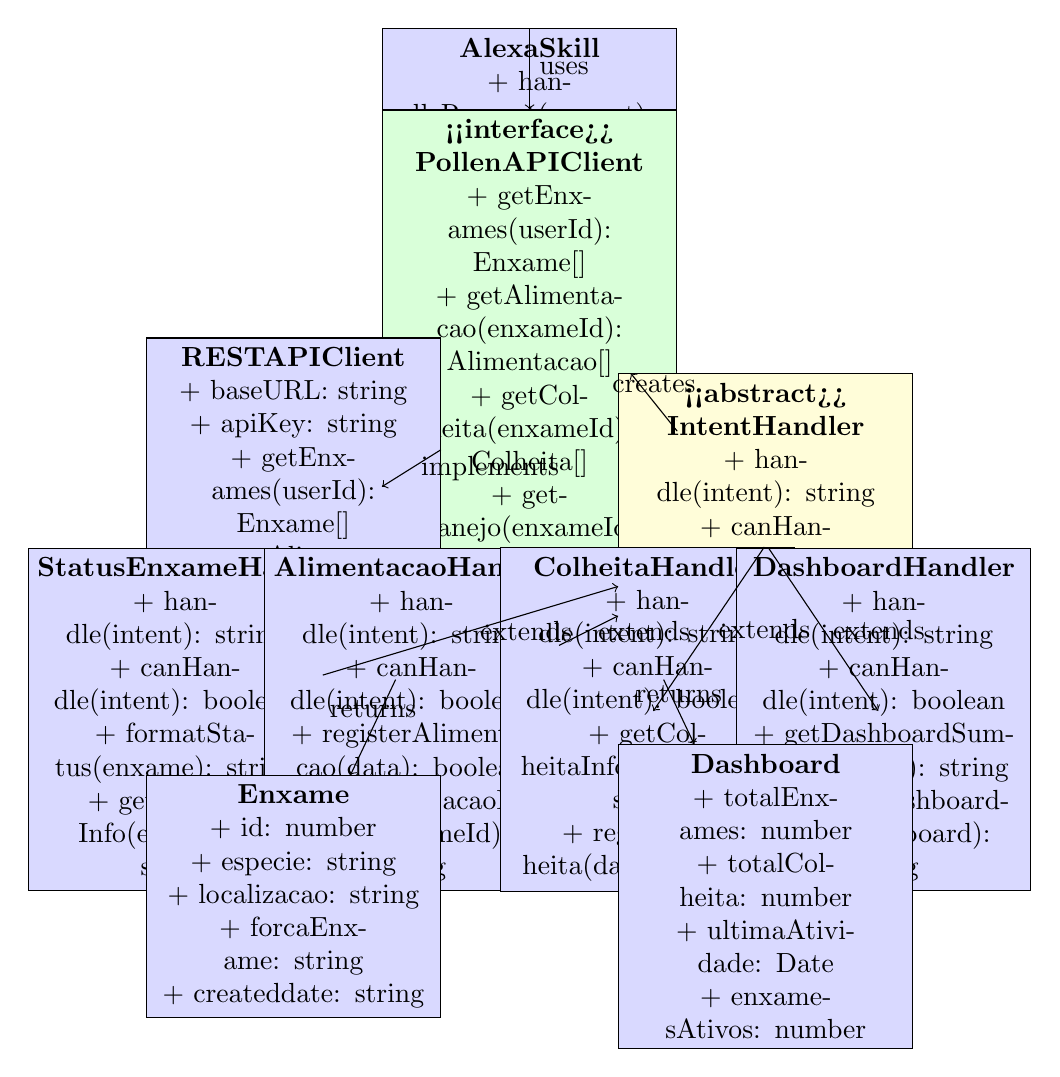
\begin{tikzpicture}[scale=0.75]
% Definição de estilos
\tikzset{
  class/.style={rectangle, draw, fill=blue!15, text width=3.5cm, text centered, minimum height=1.8cm},
  interface/.style={rectangle, draw, fill=green!15, text width=3.5cm, text centered, minimum height=1.8cm},
  abstract/.style={rectangle, draw, fill=yellow!15, text width=3.5cm, text centered, minimum height=1.8cm}
}

% Classe principal AlexaSkill
\node[class] (alexa_skill) at (0,8) {
\textbf{AlexaSkill}\\
+ handleRequest(request): Response\\
+ processIntent(intent): string\\
+ generateSSML(text): string\\
+ validateUser(userId): boolean\\
- apiClient: PollenAPIClient
};

% Interface PollenAPIClient
\node[interface] (api_client) at (0,5.5) {
\textbf{<<interface>>}\\
\textbf{PollenAPIClient}\\
+ getEnxames(userId): Enxame[]\\
+ getAlimentacao(enxameId): Alimentacao[]\\
+ getColheita(enxameId): Colheita[]\\
+ getManejo(enxameId): Manejo[]\\
+ getDashboard(userId): Dashboard
};

% Implementação RESTAPIClient
\node[class] (rest_client) at (-4,3) {
\textbf{RESTAPIClient}\\
+ baseURL: string\\
+ apiKey: string\\
+ getEnxames(userId): Enxame[]\\
+ getAlimentacao(enxameId): Alimentacao[]\\
+ makeRequest(endpoint): any
};

% Classe IntentHandler
\node[abstract] (intent_handler) at (4,3) {
\textbf{<<abstract>>}\\
\textbf{IntentHandler}\\
+ handle(intent): string\\
+ canHandle(intent): boolean\\
+ validateIntent(intent): boolean\\
\# apiClient: PollenAPIClient
};

% Handlers específicos
\node[class] (status_handler) at (-6,0) {
\textbf{StatusEnxameHandler}\\
+ handle(intent): string\\
+ canHandle(intent): boolean\\
+ formatStatus(enxame): string\\
+ getEnxameInfo(enxameId): string
};

\node[class] (alimentacao_handler) at (-2,0) {
\textbf{AlimentacaoHandler}\\
+ handle(intent): string\\
+ canHandle(intent): boolean\\
+ registerAlimentacao(data): boolean\\
+ getAlimentacaoHistory(enxameId): string
};

\node[class] (colheita_handler) at (2,0) {
\textbf{ColheitaHandler}\\
+ handle(intent): string\\
+ canHandle(intent): boolean\\
+ getColheitaInfo(enxameId): string\\
+ registerColheita(data): boolean
};

\node[class] (dashboard_handler) at (6,0) {
\textbf{DashboardHandler}\\
+ handle(intent): string\\
+ canHandle(intent): boolean\\
+ getDashboardSummary(userId): string\\
+ formatDashboardData(dashboard): string
};

% Entidades de dados
\node[class] (enxame_entity) at (-4,-3) {
\textbf{Enxame}\\
+ id: number\\
+ especie: string\\
+ localizacao: string\\
+ forcaEnxame: string\\
+ createddate: string
};

\node[class] (dashboard_entity) at (4,-3) {
\textbf{Dashboard}\\
+ totalEnxames: number\\
+ totalColheita: number\\
+ ultimaAtividade: Date\\
+ enxamesAtivos: number
};

% Relacionamentos
\draw[->] (alexa_skill) -- node[right] {uses} (api_client);
\draw[->] (rest_client) -- node[right] {implements} (api_client);
\draw[->] (alexa_skill) -- node[above] {creates} (intent_handler);

\draw[->] (status_handler) -- node[right] {extends} (intent_handler);
\draw[->] (alimentacao_handler) -- node[right] {extends} (intent_handler);
\draw[->] (colheita_handler) -- node[right] {extends} (intent_handler);
\draw[->] (dashboard_handler) -- node[right] {extends} (intent_handler);

\draw[->] (api_client) -- node[above] {returns} (enxame_entity);
\draw[->] (api_client) -- node[above] {returns} (dashboard_entity);

\end{tikzpicture}
\label{fig:classes-alexa}
\end{figura}